%%%%%%%%%%%%%%%%%%%%%%%%%%%
%                         %
%          ROOT           %
%                         %
%%%%%%%%%%%%%%%%%%%%%%%%%%%
% !TEX root = ../slides.tex

%%%%%%%%%%%%%%%
%             %
% frame begin %
%             %
%%%%%%%%%%%%%%%
\begin{frame}

%%%%%%%%%%%%%%%
%             %
% frame title %
%             %
%%%%%%%%%%%%%%%
\frametitle{The right PL for the job}

%%%%%%%%%%%%%%%%%
%               %
% itemize begin %
%               %
%%%%%%%%%%%%%%%%%
\begin{itemize}

%%%%%%%%%%%%%%%%%%%%%%%%%%%%%%%%%%%%%%%%%%%%%%%%%%%
%                                                 %
% [1] Some PLs can ``prove" their own correctness %
%                                                 %
%%%%%%%%%%%%%%%%%%%%%%%%%%%%%%%%%%%%%%%%%%%%%%%%%%%
\item<1-> Some PLs can ``prove" their own correctness

%%%%%%%%%%%%%%%%%%%%%%%%%%%%%%%%%%%%%%%%%%%%%%%%%%%%%%%%
%                                                      %
% [2] mathematical correspondance: proofs and programs %
%                                                      %
%%%%%%%%%%%%%%%%%%%%%%%%%%%%%%%%%%%%%%%%%%%%%%%%%%%%%%%%
\item<2-> Mathematical correspondance: proofs $\longleftrightarrow$ programs

%%%%%%%%%%%%%%%%%
%               %
% Itemize begin %
%               %
%%%%%%%%%%%%%%%%%
\begin{itemize}

%%%%%%%%%%%%%%%%%%%%%%%%%%%%%%%%
%                              %
% [2.i] induction -> recursion %
%                              %
%%%%%%%%%%%%%%%%%%%%%%%%%%%%%%%%
\item focus on proofs $\longrightarrow$ programs

%%%%%%%%%%%%%%%%%%%%%%%%%%%%%%%%%
%                               %
% [2.ii] induction -> recursion %
%                               %
%%%%%%%%%%%%%%%%%%%%%%%%%%%%%%%%%
\item induction $\longrightarrow$ recursion

%%%%%%%%%%%%%%%%%%%%%%%%%%%%%%%%%%%%%%%%%%%%
%                                          %
% [2.iii] translate to functional programs %
%                                          %
%%%%%%%%%%%%%%%%%%%%%%%%%%%%%%%%%%%%%%%%%%%%
\item translate to functional programs

%%%%%%%%%%%%%%%
%             %
% itemize end %
%             %
%%%%%%%%%%%%%%%
\end{itemize}

%%%%%%%%%%%%%%%%%%%%%%%%%%%%%%%%%%%%%%%%%%%%%
%                                           %
% [3] Example, finding quotient + remainder %
%                                           %
%%%%%%%%%%%%%%%%%%%%%%%%%%%%%%%%%%%%%%%%%%%%%
\item<3-> Example: Coq proof to Haskell program

%%%%%%%%%%%%%%%
%             %
% [3.i] proof %
%             %
%%%%%%%%%%%%%%%
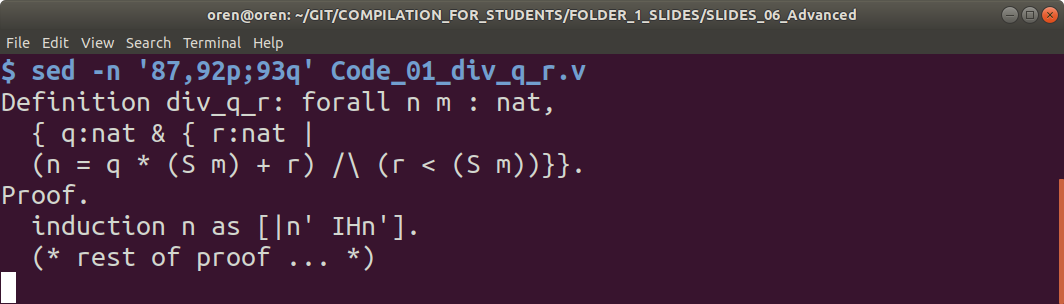
\includegraphics[width=8cm]{FOLDER_3_IMG_FILES/Code_01_div_q_r_coq.png}

%%%%%%%%%%%%%%%%%%
%                %
% [3.ii] program %
%                %
%%%%%%%%%%%%%%%%%%
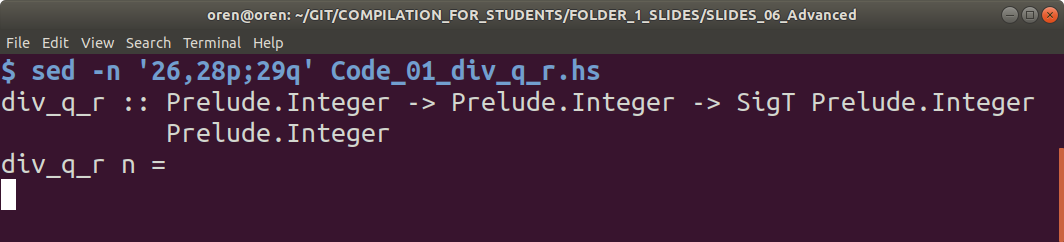
\includegraphics[width=8cm]{FOLDER_3_IMG_FILES/Code_01_div_q_r_hs.png}

%%%%%%%%%%%%%%%
%             %
% itemize end %
%             %
%%%%%%%%%%%%%%%
\end{itemize}

%%%%%%%%%%%%%
%           %
% frame end %
%           %
%%%%%%%%%%%%%
\end{frame}
